\chapter{遠端連線}
\renewcommand{\baselinestretch}{10.0} %設定行距
\pagenumbering{arabic} %設定頁號阿拉伯數字
\setcounter{page}{20}  %設定頁數
\fontsize{14pt}{2.5pt}\sectionef
\section{摘要}
  完成場景建設後,接著要實現跨網路對戰足球機器人。以 zmqRemoteAPI Python 製作控制程式,由組長開起場景,各組員分別跨網路控制各自球員進行賽局,在計時十分鐘的賽局盡可能獲得比對方更高的分數來贏得比賽。\\
\section{連線說明-防火牆}
  從控制台將防火牆都關閉,點開進階設定,組長設定"輸入規則"、組員設定"輸出規則"。新增規則 / 連接埠 / TCP(傳輸控制協定Port) / 特定連接埠 23000-23050,選擇允許連線。\\
\begin{figure}[hbt!]
\begin{center}
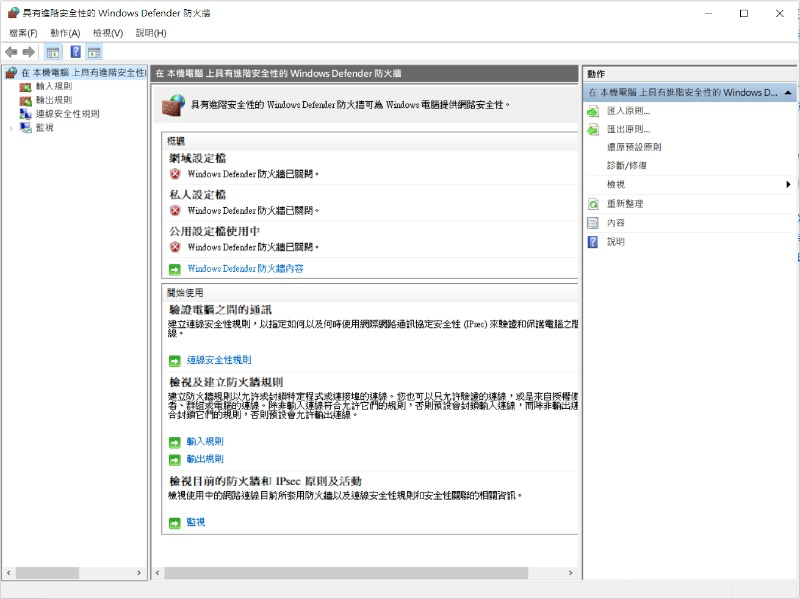
\includegraphics[height=6cm]{03}
\caption{\Large 控制台連接埠}\label{fig.03}
\end{center}
\end{figure}
\section{連線說明-IPv6}
  設定網路 IPv6 位址。\\
\begin{figure}[hbt!]
\begin{center}
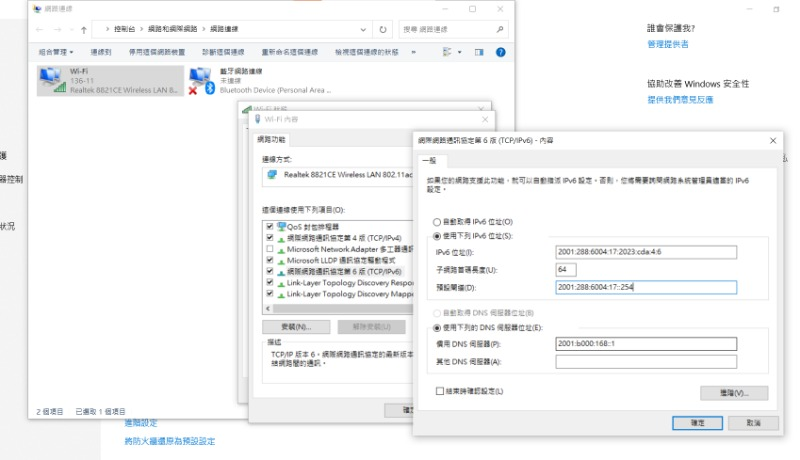
\includegraphics[height=6cm]{07}
\caption{\Large 網路 IPv6 位置}\label{fig.07}
\end{center}
\end{figure}

  下載 CoppeliaSim(4.5.1) 支援 IPv6 版本,zmq 中也需具備 IPv6 環境。\\
\begin{figure}[hbt!]
\begin{center}
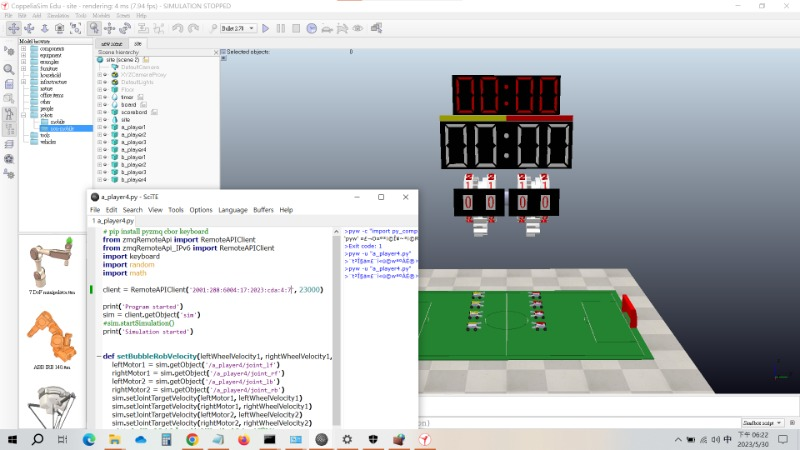
\includegraphics[height=6cm]{08}
\caption{\Large zmq IPv6 }\label{fig.08}
\end{center}
\end{figure}

  接著在 zmq 的 localhost 處打上組長的 IPv6 位置連線。\\
\newpage
\begin{figure}[hbt!]
\begin{center}
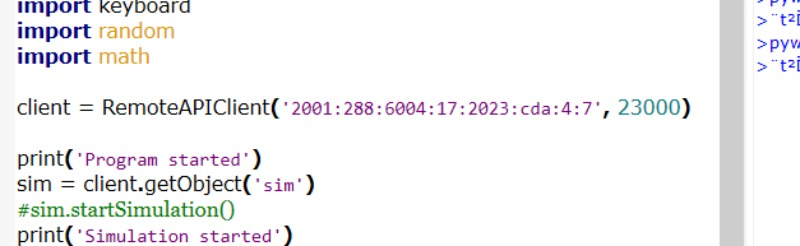
\includegraphics[height=6cm]{09}
\caption{\Large 組長 IPv6 }\label{fig.09}
\end{center}
\end{figure}
  最後在瀏覽器輸入 http://[組長 IP 位置]:23020,即可開啟網頁模擬畫面,完成 pj3 利用多輪車在一足球場景中進行對戰的目標。\\
\renewcommand{\baselinestretch}{1} %設定行距